\subsection{Adding Settings to \giraf}\label{sec:sprint3:designsettings}
The idea behind providing a way to change settings from \launcher for both itself, but also other \giraf applications, is to create a streamlined and uniform user interface for changing settings across the entire project.
This section discusses how to design the architecture of what will be an activity implemented in the context of \launcher, to contain the settings.

\subsubsection{Choosing Between Prototypes}
As discussed in \cref{sec:sprint2:secondmeeting}, the customers agreed that settings should be accessible through two methods:

\begin{itemize}
	\item A dialogue box in each individual application, containing only settings relevant to that specific application (as seen in \cref{fig:appsettingsprototype}). 
	The dialogue box should be displayed when the user presses a button identical throughout all \giraf applications, making it easier for users to find.
	\item A unified settings activity, where the user has immediate access to all settings for all \giraf applications, which should be a part of the \launcher. 
	Besides settings of individual applications, it should also contain settings available to a per-user basis, e.g. which applications the user should be allowed access to.
\end{itemize}

It is immediately apparent that for making both these approaches work in parallel, a single plan for how user settings are handled throughout the \giraf project is needed. 
In the following paragraph this plan is described.

\paragraph{Concept}
It is decided that the settings system should consist of four components, to be implemented separately:

\begin{itemize}
	\item The unified settings activity should be implemented as a part of \launcher, and therefore the implementation of this component naturally falls to ourselves. 
	Excluded from this task is the settings of the individual applications.
	\item A dialogue box able to contain the settings for an arbitrary \giraf application. Included in this is a standard button for launching the dialogue box. 
	As this User Interface component is useful to all applications, it should be implemented by the group responsible for the \giraf GUI library.
	\item A set of settings for each \giraf application.
	As these sets may vary widely in content and complexity from application to application, and furthermore may change along with their associated applications over time, these should be defined and implemented by the individual project groups. 
	\item A method for storing the settings in the database, allowing the users to easily use the same settings across several devices. 
	This should be implemented by the database group. 
\end{itemize}

\thilemann{Last item regarding remotedb - add somewhere that this is currently only done locally per device.}

\paragraph{The challenge with Implementing Settings} using the above concepts is how to allow applications other than \launcher to access the settings User Interface running in the context of \launcher as an activity.

\begin{itemize}
\item 
The first option is to ask each project group to create a \lstinline|Fragment|, which the settings activity in \launcher should be able to open.
This approach will isolate the responsibilities of each group and keep the overall complexity to a minimum.\thilemann{Why? Where to put the files and what about git? Project dependencies?}
Although there is an official way for loading a custom class\cite{customClassLoading}, it is complex and it will make the coupling of \launcher and other applications very tight.\thilemann{Does class loading even solve this???}
Additionally it is difficult to make the loading of custom classes dynamic, since the name of the class to be loaded has to be known.
The method of custom class loading is intended to be used when a project exceeds 64.000 method references, which is the limit of the Dalvik Virtual Machine.
Each Android application is running as an instance of Dalvik that sandboxes the data of the application, making it impossible for other to access it.

\thilemann{To simplify this - meaning what?}
To simplify this, \launcher has to include all other projects as dependencies when compiling, which will make the \launcher project unnecessary bloated and difficult to work with.

\item
Another possibility is to make the individual applications implement an interface, where a function would add the application's setting-widgets to a given view.
While Android provides facilities for inter-application communication through its \textit{Broadcast} mechanism\cite{broadcastReceiver}, this requires all the involved applications to be running.
This is not an acceptable condition in this situation. 
\end{itemize}
 
\subsubsection{A title saying that this is our decision}\thilemann{Fix title!}
Instead of the to presented options above, another design is chosen.
An Android feature called Intent Filters allows applications to request an action from another \textit{app component}; an activity, a broadcast receiver, a content provider or a service.
It is implemented by adding \lstinline|<intent-filter>...</intent-filter>| to the Android Manifest with its actions (or intentions) defied within.\cite{intentFilter}
With this method it is possible to check each installed application to see if it implements a certain action (which will be the same for each \giraf application implementing the Intent Filter).
If an application implements this filter, it can be assumed that it provides an activity for showing settings, which in turn can be added safely to the list in the settings activity of \launcher.

With this design it is not possible to load settings from other applications as fragments in our application. Instead we start their application and their settings.
However, this simplifies the complexity about saving the settings.
If we were to load their settings as a fragment we were loading the settings in context of our application. 
Meaning that we save the settings again in our context and we have to figure out a solution for them to load the settings from our context.

\subsubsection{Designing from Prototypes}

\begin{figure}[h]
\centering
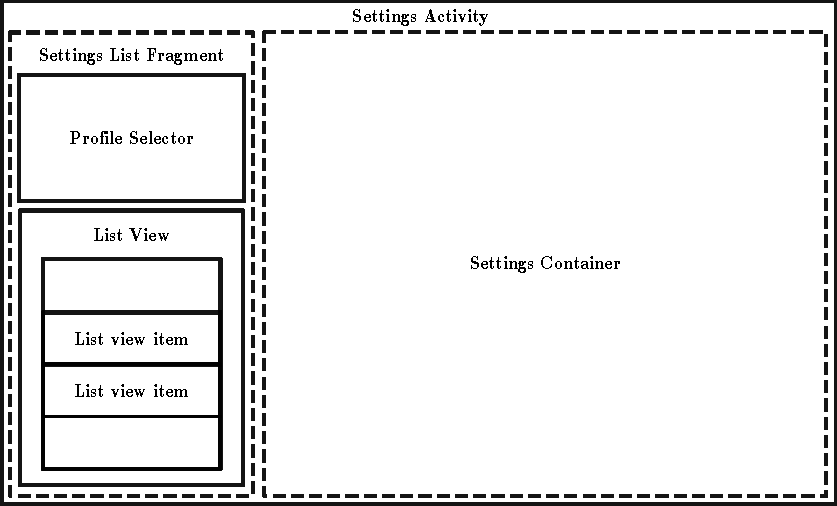
\includegraphics[width=\textwidth, keepaspectratio=true]{SettingsActivity.pdf}
\caption{The architecture showing how the prototype, \cref{fig:settingsprototype}, will be implemented.}
\label{fig:settingsarchitecture}
\end{figure}

Having investigated how to handle settings from other \giraf applications in \cref{sec:sprint3:designsettings}, this sections elaborates on how this is designed following Android terminology taking \cref{fig:settingsprototype} as the underlying basis of the design decisions.

\paragraph{Settings Activity}
Analogous to opening a new window on a desktop computer, a ``screen'' on an Android device consists of an activity.
\Cref{fig:settingsprototype} can be compared directly to \cref{fig:settingsarchitecture}, to expand on the User Interface components that need be included.

To follow Android guidelines we are using fragments\cite{fragments} to implement the functionality this activity requires. They are reusable modules which gives decomposition of the application functionality and UI. By using fragments it is also possible to add multiple fragments to a screen without switching activity.

By following these guidelines for developing an activity it is possible to use the same implementation to show the settings on a smaller screen, this is not a requirement at the moment and therefore this has not been taking into account.\\

As illustrated in \cref{fig:settingsarchitecture} it consists of one fragment, \textbf{Settings List Fragment}, and one container, \textbf{Settings Container Fragment}.
The settings list fragment contains the profile selector and a list view, these are described below
\begin{itemize}
\item \textbf{Profile Selector} is what makes it possible to edit settings for multiple users.
The prototype previously mentioned shows a profile selector resembling a drop-down menu.
To follow the multi-project guidelines, a component developed by the group responsible for the GUI library will be implemented instead.
When the selected profile changes, settings activity should be reloaded to reflect the newly selected user's settings.
\item \textbf{ListView} shown the categories of settings which are available for the user.
The fragment attached to each category is presented in the settings container fragment when the category is chosen.
\end{itemize}
























